\chapter{Background}
\label{ch:background}

In this chapter, we present the background that (...)

\section{Hydra Algorithm}
\label{sec:hydra_algo}
Hydra \cite{Dempster2023Hydra} - which stands for \textbf{HY}brid \textbf{D}ictionary-\textbf{R}ocket \textbf{A}rchitecture - is a time-series classification algorithm, and it is a cross between two sub-families of such algorithms: dictionary methods and random convolutional kernels (RCK).
The proponent authors, Dempster et al., have a track record in RCK algorithms, being the original proponents of both Rocket \cite{Dempster2020} and MiniRocket \cite{Dempster2021MR} algorithms, which were the first of its kind,
and were characterised by retaining a similar accuracy to state-of-the-art methods, but requiring only a fraction of the computational effort. They are inspired in convolutional neural networks, but they instead rely on a large number of convolutions with fixed, but randomized, weights.
On the other hand, dictonary methods, using the same windowing approach as before, approximate an input time series as a "word", which is composed of "letters" that represent the occurence of a given pattern. The occurence of words is used to build up a histogram.

Hydra merges these two approaches, by using the RCK, competing between themselves, to form words, which are then accumulated over the length of the input time series to form a histogram, like dictionary methods, which serve as the input to a linear classifier. It only differs from dictionary methods
in the way it extracts the temporal patterns.

In the following sections, a more detailed overview of this algorithm is presented. We start by laying out the background of the methods that inspired hydra in Section \ref{sec:ha_related_work} in a high-level conceptual manner, and then provide a more rigorous and analytical formulation fro Hydra in Section \ref{sec:ha_algo_descr}.

\subsection{Related Work}\label{sec:ha_related_work}
\subsubsection{Random Convolutional Kernels}{sec:ha_rck}
Convolutional Neural Networks (CNNs) have long shown effectiveness in image classification, and \cite{Fawaz2020} notes, with the proposal of "InceptionTime", that this is likely to also be the case with the more generic task of time-series classification, which is a one-dimensional problem instead of the two-dimensional problem of image classification.
The main principle is that the kernel weights learn unique features from the data, making each class separable in the resulting feature map space, because the most similar a given pattern is with a given window of the input time signal, the larger the output will be, and vice-versa. This can be seen with the basic CNN formula

\begin{equation}\label{eq:basic_cnn_eq}
y[n] = \sum\sb{k=0}\sp{K} w[k] \cdot x[n+k]
\end{equation}
where $y[n]$ is the convolutional output at time instant $n$. The ouptut $y[n]$ is larger (in absolute value) the more $w$ and $x$ are similar in shape. Suppose, for instance, that $w[n]$ is constant and $x[n]$ is sinusoidal with one or more full periods contained within the kernel stride: in that case $y[n]$ would be zero.

CNNs extend this principle, by realizing that some patterns might not be local to the kernel stride, but might exist across \textbf{longer scales} of the input time series. Towards this purpose, they make use of \textbf{dilations}, where a number $d$ of samples from the input sequence $x[n]$ is skipped in the computation of the convolution
output $y[n]$. In analytical terms, this can be achieved with the reformulation of Equation \label{eq:basic_cnn_eq} such as

\begin{equation}\label{eq:dil_cnn_eq}
y[n] = \sum\sb{k=0}\sp{K} w[k] \cdot x[n+ d \cdot k].
\end{equation}
Lastly, CNNs also use \textbf{padding} at the edges of the input sequence $x[n]$, by adding zeros to the beginning and end of the sequence, such that the weight at the middle of the kernel aligns with the \emph{first sample} of $x[n]$ at the \emph{start} of the operation, and with the \emph{last sample} at the \emph{end} of the operation.

Random Convolutional Kernels build upon these ideas, but have a fundamental difference: while weights in CNNs are trained to better approximate the characteristic shapes in the input data, RCKs use \textbf{fixed}, but \textbf{random} weights, which do not need a training phase, and rely on the fact that having a large number of them will eventually
use the most relevant kernels. This idea was initially explored in CNNs by \cite{Saxe2011random}, albeit using an Support Vector Machine as a classifier. 
Furthermore, \cite{Dempster2020} suggests that, as with other similar data intensive methods, CNNs need a large ammount of data of properly learn the kernel weights that best approximate the features to extract from the input time series, and that results like those of \cite{Fawaz2020} show high variance on the classification accuracy of the datasets
if the UCR archive with the least amount of training examples. For a full discussion on the history and other usages of RCKs, refer to \cite{Dempster2020}.

Lastly, we would like to discuss the most recent RCK-based time-series classification works that most resemble Hydra, and from which Hydra took its inspiration: they are Rocket \cite{Dempster2020}, proposed in 2020, and MiniRocket \cite{Dempster2021MR}, proposed in 2021.

Rocket \cite{Dempster2020} implements a series of RCKs that operate in parallel in a single layer. The computation for all RCKs is then repeated across all the hyperparameters of these kernels are also randomized, namely the kernel length (from the set ${7, 9, 11}$), the padding legths and the bias value applied to the convolution ouputs. 
As each of the RCKs is convolved with the input time series, a convolutional output is produced for each of the input samples, such that the output, $y[n]$ has the same length as the input $x[n]$. Since this would result in a very large data vector, each of these kernel outputs $y[n]$ is transformed into a group of \textbf{two} features
Then, for each combination of these hyperparameters, each RCK will produce a group of features by separately applying two \textbf{non-linear} functions that map the full output length to a single value. These functions are the \textbf{maximum} value, and the \textbf{proportion of positive values}, PPV,  of each RCK convolution. We should emphasise that these
non-linearities are applied to \emph{each combination of RCKs and hyperparameters separately}, so that the resulting feature vector has \emph{twice} as many features as the product of the number of RCKs used and the number of each of the possible hyperparameters used - as reported in \cite{Dempster2020}, their implementation produces 2k features
per input time series, whose computation is repeated across 10k RCK kernels, which yields a total of 20k features. This feature vector is then used as the training inputs to a linear classifier, such as Logistic Regression or Ridge Regression.

MiniRocket \cite{Dempster2021MR}, proposed by the same authors of Rocket, attemps to simplify its formulation, by removing unnecessary aspects that improve little to nothing on the model accuracy. 
The most striking changes, are the use of kernels of only one length, 9, using weight values from a set of only two values, -2 and 1 (instead of sampling them from a standard normal distribution, retrieving the bias from the convolutional output, using fixed dilation values instead of sampling them and, lastly, only using the PPV feature for constructing the feature vector, instead of also using the maximum like in MiniRocket.
Moreover, the authors propose that, instead of sampling the weight values from the set ${-2, 1}$, to build a \emph{permutations} of these two values for kernels of size 9, such that all possible combinations are accounted for. 
After this, like in Rocket, the computation of these kernels is repeated for all combinations of the hyperparameters. As for Rocket, this feature vector is also used as the training input to a linear classifier.

\subsubsection{Dictionary Methods}
As mentioned before, dictionary methods work, as their name suggests, by sliding an analysis window over the input time series, and by forming ``words'' for each of these windows, whose letters represent the occurence of given characteristic patterns.
The occurrence of each word is accumulated in a \tetxbf{histogram}, which is then used to train a classifier. 
For a full discussion on the history and usages of dictionaries, the reader can refer to \cite{Dempster2020}. 
The discussion of the minute details of each algorithm is out of scope for this work, since the meaningful background to understand Hydra is the general concept of how dictionary methods operate.

\subsubsection{Hydra}
Hydra builds upon the notions of the two previous sections. It is a dictionary method in the sense that it makes a statistic of the pattterns that are extracted, but those patterns are extracted in a ``Rocket''-like fashion, since the dictionary letters are formed with the outputs of the RCK.
Now, the way in which the RCK outputs are transformed into words is done in a specialized way, in that instead of being each by themselves separately, they are instead organized into \textbf{groups}, within which they compete to be the chosen ones, at each time step, to be accounted for in the dictionary-like histogram.

\subsection{Algorithm Description}\label{sec:ha_algo_descr}
A more rigorous analytical description is provided here. The algorithm is comprised of three stages, which will be detailed in Sections \ref{sec:ha_s1}-\ref{sec:ha_s3}.
The typical way in which Hydra is used, in terms of which stages need training, and where the results of this training are using at inference time
are summarized in Figure \ref{fig:overview_hydra}
\begin{figure}[h!]
\begin{tikzpicture}[x=1cm,y=1cm]
	\coordinate (scal_training_cote) at (0,0); 
	\coordinate (clas_training_cote) at (0,-2); 
	\coordinate (inference)          at (0,-4); 

	\draw [blue,thick] ($(scal_training_cote) +  (0,0)$) node[fill=yellow!80!black,align=center] (ids) {Input Data \\ $N \times L_x$};
	\draw [blue,thick] ($(scal_training_cote) +  (4,0)$) node[fill=yellow!80!black,align=center] (tfs) {Feature Vector \\ $N \times F$};
	\draw [blue,thick] ($(scal_training_cote) +  (9,0)$) node[fill=yellow!80!black,align=center] (msd) {Mean and Std. Dev. \\ $2 \times N \times F$};

	\draw [blue,thick] ($(clas_training_cote) + (4,0)$) node[fill=yellow!80!black,align=center] (scf) {Scaled Features \\ $N \times F$};
	\draw [red,thick] ($(clas_training_cote) + (11,0)$) node[fill=yellow!80!black,align=center] (clf) {Classifier \\ Training};

	\draw [blue,thick] ($(inference) +  (0,0)$) node[fill=yellow!80!black,align=center]  (its)  {Input Series \\ $1 \times L_x$};
	\draw [blue,thick] ($(inference) +  (4,0)$) node[fill=yellow!80!black,align=center]  (stfs) {Feature Vector \\ $1 \times F$};
	\draw [blue,thick] ($(inference) +  (8,0)$) node[fill=yellow!80!black,align=center]  (sscf) {Scaled Features \\ $1 \times F$};
	\draw [blue,thick] ($(inference) + (11,0)$) node[fill=yellow!80!black,align=center] (sprd) {Prediction};

	\draw[->] (ids) edge node[above] {Step 1} (tfs);
	\draw[->] (tfs) edge node[above, align=center] {Calculate \\ Mean and Std} (msd);
	\draw[->] (msd) edge node[above] {$\frac{X-\mu}{\sigma}$} (scf);
	\draw[->] (msd) edge node[above] {$\frac{X-\mu}{\sigma}$} (sscf);
	\draw[->] (scf) -- (clf);

	\draw[->] (its)  edge node[above] {Step 1} (stfs);
	\draw[->] (stfs) edge node[above] {Step 2} (sscf);
	\draw[->] (sscf) edge node[above] {Step 3} (sprd);

	\draw[dashed] ($(scal_training_cote)+(-2,1)$) -- ($(scal_training_cote)+(0,1)$) node[above] {\textbf{A.} Scaler Training} -- ($(scal_training_cote)+(12,1)$); 
	\draw[dashed] ($(clas_training_cote)+(-2,1)$) -- ($(clas_training_cote)+(0,1)$) node[above] {\textbf{B.} Classifier Training} -- ($(clas_training_cote)+(12,1)$); 
	\draw[dashed] ($(inference)+(-2,1)$)          -- ($(inference)+(0,1)$)          node[above] {\textbf{C.} Inference} -- ($(inference)+(12,1)$); 

\end{tikzpicture}

\caption{Overview of Hydra}
\label{fig:overview_hydra}
\end{figure}
\subsubsection{Stage 1: Random Convolutional Kernel Transform}\label{sec:ha_s1}

\begin{itemize}
    \item Convolutional Outputs $y\sb{[k,h,d]}[i] = \sum\sb{j=0}^{W-1} x[i+j\dot d] w[j]$, repeated for all $d \in [1,D-1]$.
    \item Feature Vector Update
        \begin{itemize}
            \item Hard Counting (Min): $F\sb{[h,d]}[2k+0] += 1$,              where $k = \text{argmin}\sb{k} (y\sb{[k,h,d]}[i])$.
            \item Soft Counting (Min): $F\sb{[h,d]}[2k+1] += y_{[k,h,d]}[i]$, where $k = \text{max}\sb{k} (y\sb{[k,h,d]}[i])$.
        \end{itemize}
    \item Repeat previous steps for $i \in [0, L_x-1]$. 
\end{itemize}
Note that the value of the convolutional output for the input sample at index $i$ is independent of the outputs at any other index.
This means that we \textbf{do not} need to store all values of $y_{[k,h,d]}[i]$. Each update of the feature vector $F$ requires only $k \in [0,K-1]$ outputs at index $i$ of $y$.

\subsubsection{Stage 2: Sparse Scaling}\label{sec:ha_s2}
\begin{itemize}
    \item $F\sb{[:,:,:]}[i] = \frac{\text{clip}(F\sb{[:,:,:]}[i],0) - \mu[i]}{\sigma[i]}$, if $\text{clip}(F\sb{[:,:,:]}[i],0) > 0$
    \item $\mu$ and $\sigma$ are arrays of size $L_F$, trained with the transformed training set.
\end{itemize}
\subsubsection{Stage 3: Classifier}\label{sec:ha_s3}
\begin{itemize}
    \item $\text{argmax}\sb{c} (Q[c])$, where $Q = B \cdot F$, and  $B \in \mathcal{M}\sb{C \times L_F}$.
\end{itemize}

\section{UCR Archive Dataset}
The UCR Time Series Classification Archive \cite{UCRArchive2018} is specialized collection of datasets for time-series classification problems. 
They contain both synthetic and real data, and the samples are all comprised of a sequence of values. This sequence is not always temporal, as there is also
spectral data - in which case the samples correspond to the spectral bin values, that although not temporally related maintain an inter-sample dependency like time series data;
some of the so-called ``image'' data is generally a \textbf{post-processed} version of an image, transformed in some way to become a 1-d data sequence that fits the problem formulation 
(e.g. in the ``Fish'' dataset, an 2d outline is extracted from the fish image, which is then projected into 1-d space to form the input sequence data that is actually part of the dataset).

This collection is very useful for evaluating time-series classification algorithms for a number of reasons, namely:

\begin{itemize}
    \item \textbf{Large variety of problems} -- the large variety of types of data test an algorithms ability to perform well across many distinct tasks. The types of problems are (as reported from \cite{UCRArchive2018}):
        \begin{itemize}
            \item Audio
            \item Device (e.g. power consumption profile)
            \item ECG, EEG, EMG, EOG
            \item Financial
            \item Human Activity Recognition
            \item Hemodynamics
            \item Image
            \item Other sensor data
            \item Simulated
            \item Spectral data
            \item Speech
            \item Traffic
        \end{itemize}
    \item \textbf{Small number of training samples} -- most datasets contain less than 1k training samples, which is a challenge for an algorithm's ability to learn from limited data. Data intensive algorithms might struggle to achieve high accuracy without resorting to data augmentation.
    \item \textbf{Test/Train Split exceptionally hard} -- is most datasets, the training set is either the same size as the test set, or even considerably smaller. This is an excellent test to an algorithm's ability to generalize and avoid over-fitting to the training data.
\end{itemize}
It is obvious that some of this data, although being strictly speaking time-series data, it is considered out-of-scope for our specific problem of TinyML embedded applications, which generally deals with streams of sensor data. Still, the UCR Archive is used as a general benchmark for a model, not for specific embedded applications.
It is up to the author of a given TinyML model the ascertain its fitness to a specific problem based on how it performs on across that specific subset of datasets in the UCR Archive.

\section{GAP9 Microcontroller}

Lastly, we provide a brief discussion about the chosen deployment platform, the GAP9 microcontroller \cite{GWGAP9}. 
It is a micro-processor tailored for low-power, high-performance embedded applications, with state-of-the-art power consumption. It is a RISC-V architecture

\begin{figure}[h!]
    \centering
    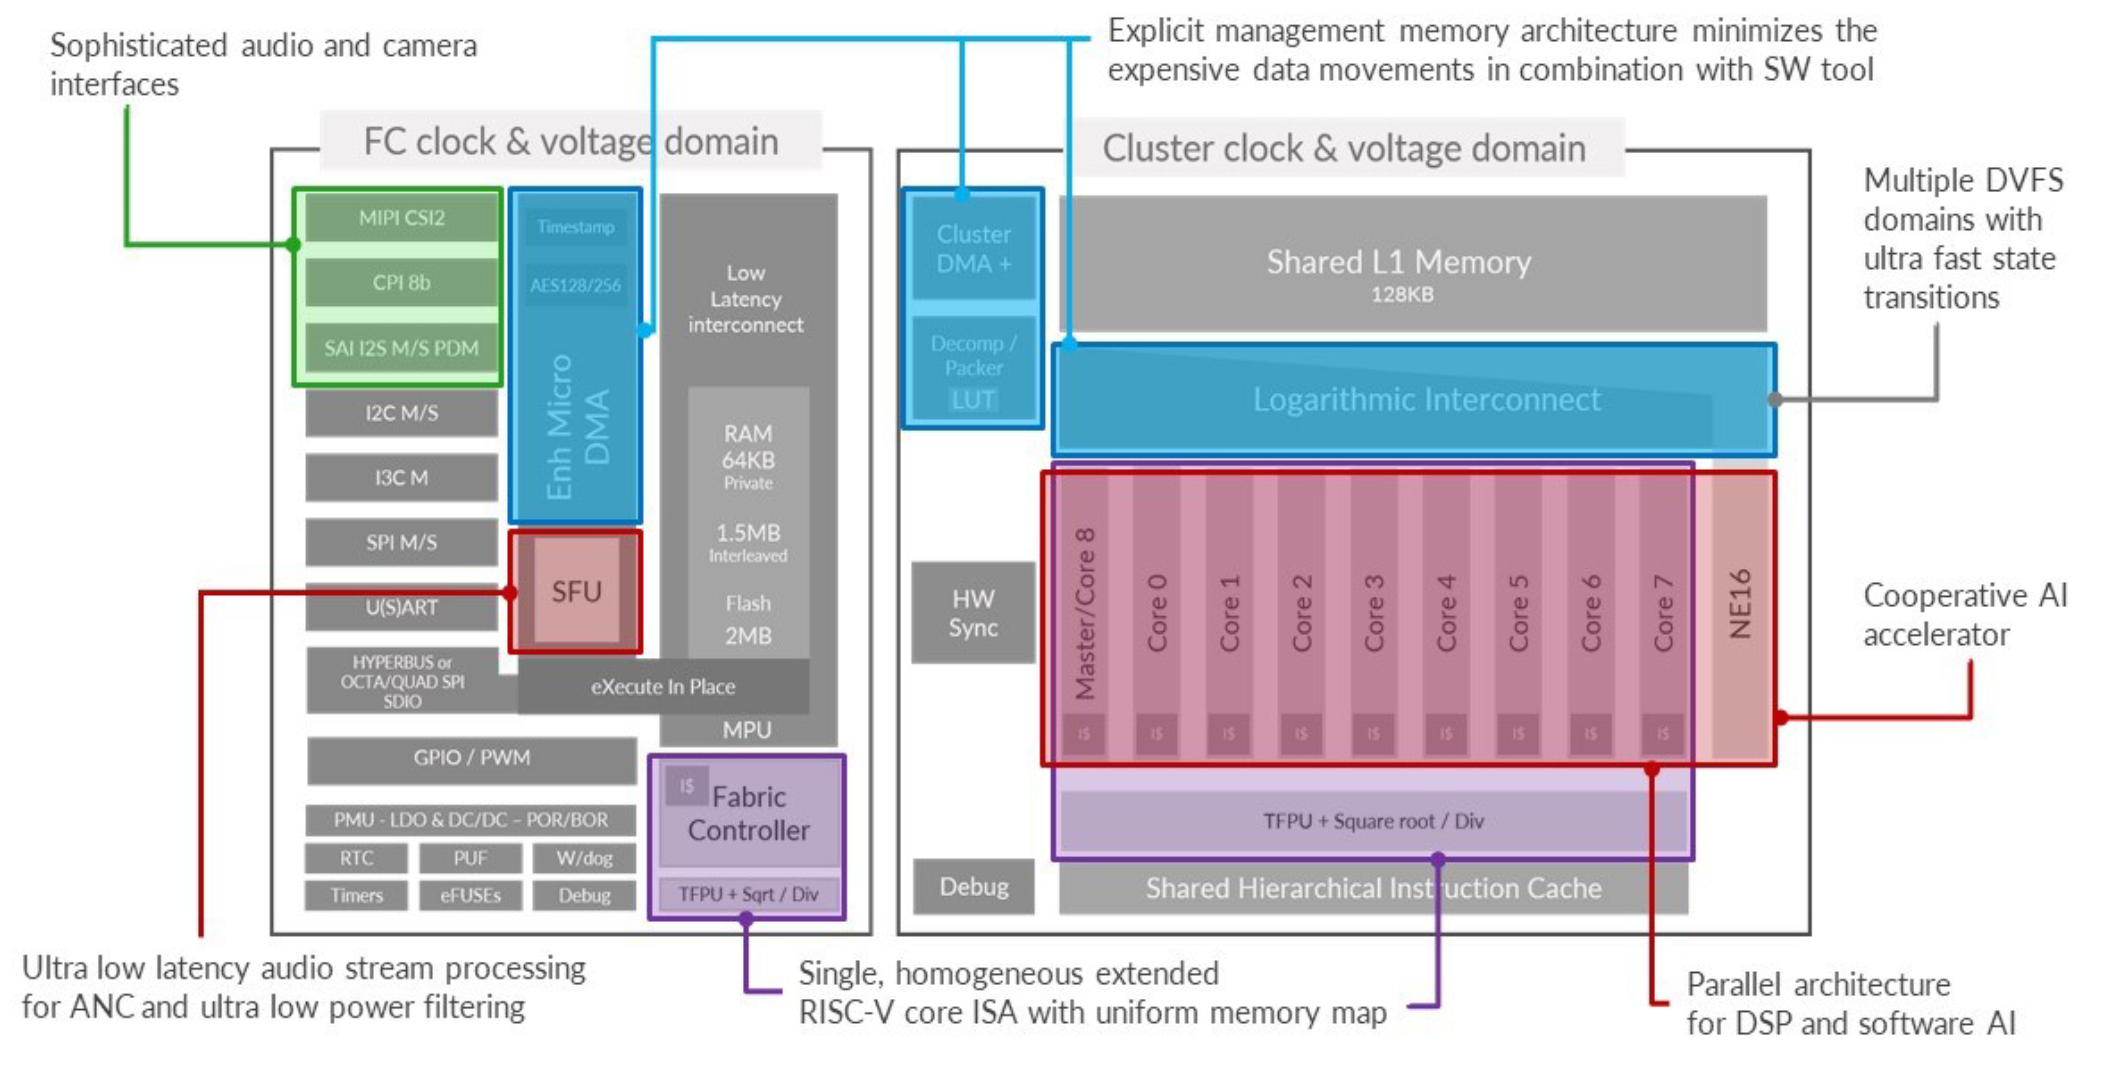
\includegraphics[width=\textwidth]{fig/gap9_toplevel.png}
    \caption{Top-level architecture of the GAP9 Processor. Picture reproduced here from the product brief in \cite{GWGAP9}}
    \label{fig:gap9_toplevel}
\end{figure}